\documentclass[12pt, a4paper, lithuanian, final]{article}

\usepackage{hyperref}
\usepackage{graphicx}
\usepackage{float}
\usepackage{placeins}
\usepackage{gensymb}
\usepackage{xcolor}
\usepackage{listings}
\usepackage{amsmath}
\usepackage{textgreek}
\usepackage{mathtools}
\usepackage[obeyFinal]{easy-todo}
\usepackage[utf8]{inputenc}
\def\LTfontencoding{L7x}
\usepackage[\LTfontencoding]{fontenc}
\usepackage[lithuanian]{babel}
%\usepackage{times}

%\renewcommand{\sfdefault}{uhv}
%\renewcommand{\rmdefault}{utm}
%\renewcommand{\ttdefault}{ucr}

\usepackage{VUMIF}

%Kodo highlitinimo configas
\lstset{basicstyle=\ttfamily,
	showstringspaces=false,
	commentstyle=\color{red},
	keywordstyle=\color{blue}
	}


% Titulinio puslapio reikalai
\vumifdept{Programų sistemų katedra}
\vumifpaper{}
\title{Praktikos UAB "`Elektromotus"' ataskaita}
\author{
    4 kurso 1 grupės studentas \\
    Rytis Karpuška
}

\supervisor{Irus Grinis, lekt.}
\reviewer{Karolis Tarasauskas}
\date{Vilnius \\
	2015}


\begin{document}

%titulinis ir turinys
\maketitle
\tableofcontents

\vumifsectionnonum{Įvadas}

Įterptinėmis sistemomis, jų kūrimu, bei programavimu domiuosi jau daugelį metų, todėl nenuostabu, kad praktiką pasirinkau atlikti įmonėje siejančioje savo veiklą su tokiomis sistemomis.
Uždaroji Akcinė Bendrovė "`Elektromotus"' yra viena iš nedauglio įmonių kurianti ir parduodanti įterptinių sistemų produktus.
Tiesa, šioje įmonėje dirbu jau ketverius metus, todėl darbas čia nebuvo nauja patirtis.
Tai yra viena iš pagrindinių šios vietos pasirinkimo priežaščių, tačiau nevienintelė, taip pat labai svarbu, kad įmonė vykdo nevieną įdomų projektą.
Pradėdamas praktiką, kartu su komanda, vieną iš projektų vysčiau apie metus, buvo sukurta techninė ir programinė įranga, bet pasirodė, kad testavimo procedūros turėjo stiprių trūkumų.
Todėl savo praktikos atlikimui išsikėliau uždavinį patobulinti šio projekto testavimo procedūras.


\paragraph{Praktikos Užduotis}

Įmonė nekaupia istorinių duomenų apie ankstesnius defektus, bet yra aiškiai matomas įterptinių sistemų testavimo proceso neapibrėžtumas, matomi atliekamo testavimo trukūmai, bei defektai patenkantys į produkcinį kodą.
Todėl savo praktikoje išsikėliau tokius uždavinius:
\begin{itemize}
	\item Patobulinti regresinį vienetų testavimą, sukurti principus, pagal kuriuos šis testavimas įmonėje būtų atliekamas dažniau
\end{itemize}

Įmonėje buvo atliekami vienetų testai ir ankščiau, bet jų vykdymas buvo sudėtingas ir nesistemingas, dėl ko kartais nevisada būdavo pastebimos vienetų testų klaidos, pasitaikydavo situacijų, kuomet vienetų testai būdavo apleidžiami visai.

\begin{itemize}
	\item Sukurti programinius modulius skirtus pagreitinti ir palengvinti programų derinimą įmonės kuriamuose produktuose
\end{itemize}

Įterptinių sistemų derinimas yra sudėtinga užduotis, kurią dar labiau apsunkina menki tokių sistemų resursai, labai apribotos sąsajų galimybės, neretai pasitaikantys labai aukšti reikalavimai vykdymo laiko tikslumui.











%Skyrius apie įmonę
\section{Apie UAB "`Elektromotus"'}

UAB "`Elektromotus"' 2010 metais įkurta trijų steigėjų: Gintauto Palucko, Mindaugo Milašausko ir Šarūno Šutavičiaus su tikslu realizuoti jų sukauptą patirtį elektromobilių valdymo sistemų kūrimo srityje.
Nuo to laiko, įmonė išaugo ir samdyti darbuotojai pilnai perėmė įmonės darbo krūvius.
Šiuo metu įmonėje yra 15 darbuotojų, metinė apyvarta viršyja milijoną litų, bei vykdomas ne vienas naujas projektas, su tikslu, patobulinti, išleisti, sukurti naujas technologijas bei produktus.

Buvo sukurti ir išleisti keli produktai, bei patentai.


\subsection{Produktai}
\subsubsection{"`Emus BMS"' -- baterijų valdymo sistema}
"`Emus BMS"' yra pagrindinis ir seniausias įmonės produktas, įnešantis daugiausiai pajamų.

Tai yra valdymo sistema vidutinėms ir didelėms ličio jonų, ličio polimerų, ličio geležies fosfatų, nikelio-metalo hidratų ir kitoms baterijoms.

Sistemą sudaro trijų lygmenų hierarchinė struktūra:

\begin{figure}[H]
\begin{center}
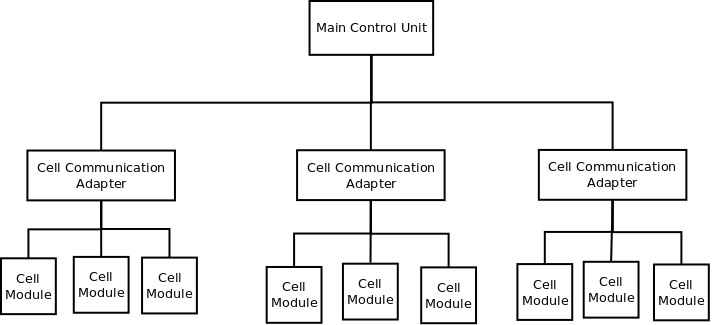
\includegraphics[width=1\textwidth]{img/bms_desc.png}
\caption{Emus BMS struktūra.}
\end{center}
\end{figure}

Sistemą sudaro šie komponentai:
\begin{itemize}
	\item{\textit{Main Control Unit}} -- pagrindinis valdymo blokas komunikuojantis su komunikacijos adapteriais CAN sąsaja.
	\item{\textit{Cell Communication adapter}} -- adapteris persiunčiantis CAN sąsajos komandas į celių modulius privačia įmonės sukurta sąsaja pritaikyta dirbti EMI triukšmingose sąlygose.
	\item{\textit{Cell module}} -- celių moduliai, galiniai įrenginiai, matuoja celės įtampą, temperatūra, turi šiluminio balansavimo palaikymą.
\end{itemize}

Panašių sistemų rinkoje labai mažai, tad ši sulaukė populiarumo.
Ši sistema yra naudojama įvairiuose elektromobiliuose, laivuose, kranuose. ir t.t.

Ryškiausi klientų pasiekimai su "`Emus BMS"':
\begin{itemize}
	\item Komandos "`ACCIONA"' bolidas dalyvavęs "`Dakar"' ralyje.
	\item Academic Motorsports Club Zurich (AMZ) automobilis, pasiekęs 100km/h per 1.785s, taip sumušdamas pasaulio rekordą.
	\item "`Intersolar 2013, Munich"' saulės jegainės valdikliuose.
	\item "`EcoPower Hybrid"' kranas, dirbantis Teksaso uoste.
	\item "`Lloyds paxter"' pašto elektromobiliuose Norvegijoje.
\end{itemize}











%Skyrius apie mano veiklą įmonėje
\section{Veikla praktikos metu}

Praktikos metu įmonėje dirbau prie naujo įmonės projekto.
Projekto metu buvo sukurta sensorių sistema, skirta geležinkelių aukštos įtampos kabelio vibracijoms tirti.
Sistema atitinka Šeimininko-Vergo (ang.: \textit{Master-Slave}) topologiją, leidžiančią vienu metu palaikyti iki 16 sensorinių tinklo mazgų.

\begin{figure}[H]
\begin{center}
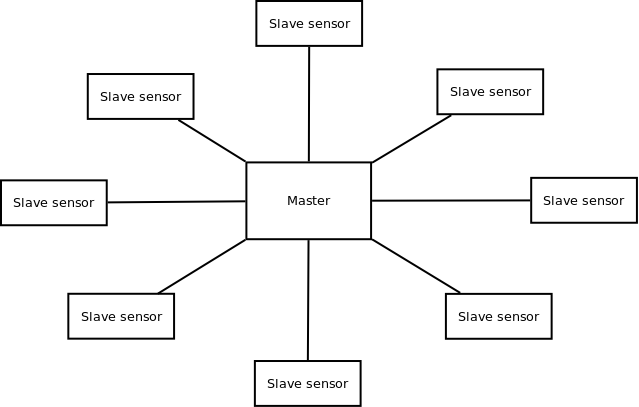
\includegraphics[width=1\textwidth]{img/NorgeRail_star.png}
\caption{Vibracijų sensorių tinklo topologija su 8 sensoriais.}
\end{center}
\end{figure}

\begin{itemize}
	\item \textit{Slave} -- moduliai matuojantys akseleracijas visomis trimis kryptimis ir komunikuojantys su "`Master"' moduliu
	\item \textit{Master} -- modulis valdantis visą sistemą, priimantis matavimo duomenis, suteikiantis internetinę prieiga sistemos konfigūravimui, stebėjimui bei matavimų parsisiuntimui
\end{itemize}

Šio projekto metu dėl labai aukštų elektros suvartojimo ir duomenų perdavimo greičio reikalavimų nuo pagrindų buvo sukurtas žvaigždės topologijos radio tinklas.
Suprogramuotas specialus laiko dalinimosi algorithmas ramiom darbo sąlygom leidžiantis techninę radio ryšio įrangą įjungti mažiau nei 1\% laiko, taip sutaupant elektrosr. Atmetus visus protokolo nuostolius per vieną kanalą pasiekiamas 15KB/s srautas daugiau kaip 1 kilometro atstumu (jeigu tarp "`Master"' ir "`Slave"' įrenginių nėra fizinių kliūčių).

Šie algoritmai buvo pakankamai efektyvūs, kad"`Slave"' sensoriai be pertraukų atliktų matavimus 7 dienas iki baterijos išsikrovimo.


Negana labai aukštų reikalavimų elektros suvartojimui, šie sensoriai turi stabiliai dirbti labai EMI triukšmingoje aplinkoje, nes jie montuojami teisiogiai ant aukštos įtampos kabelio.
Tam buvo sukurtas specialus faradėjaus narvo savybes imituojantis korpusas apsaugantis vidinę elektroniką.


"`Master"' įrenginyje dirbo Linux operacinė sistema, kuriai buvo atskirai parašytos tvarkyklės privačiam šios sistemos protokolui palaikyti.
Taip pat įrenginys buvo aprūpintas Wi-Fi ir GSM sąsajom, todėl parsisiųsti matavimus, stebėti kaip sistema dirba, o prireikus perkonfigūruotis "`Slave"' bei "`Master"' įrenginius galima nuotoliniu būdu.



\subsection{Naujos Testavimo procedūros}


Prasidėjus profesinei praktikai projektas jau buvo pažengęs ir buvo atlikti bandymai realiuose geležinkeliuose Trondheim ir Oslo traukinių stotyse, Norvegijoje.
Deja, bandymai parodė, kad sistemoje buvo nemažai programinės įrangos defektų, tame tarpe ir kritinių, dėl kurių buvo įmanoma pilnai prarasti ryšį su "`Slave"' sensoriais.
Todėl buvo nuspręsta, kad reikia sustiprinti testavimo procedūras.

\subsubsection{Regresiniai vienetų testai}


Vienetų testai (ang.: \textit{Unit tests}) įmonėje buvo vykdomi ir ankščiau, bet, deja, darbas su jais buvo varginantis ir nepatogus.
Vien jų paleidimas reikalavo specialios įrangos, kad pavyktų prijungti programuojamą įrenginį prie kompiuterio,
testai turėdavo būti paleidinėjami rankomis. Reikėjo įvedinėti lengvai pamirštamas komandas.
Testus pernešti iš vieno projekto (kodo bazės) į kitą būdavo labai sunku, tad kai kurie seniau parašytų modulių testai būdavo ištrinami norint greičiau pasiekti sėkmingą kompiliaciją.
Yra pasitaikę situacijų, kai testai buvo išvis apleisti ir neatnešė realios naudos.
Šių vienetų testų tikrai nebuvo galima pavadinti regresiniais, o tai yra viena iš stipresnių vienetų testų savybių.

Todėl po nesėkmingų sistemos bandymų Norvegijoje buvo nuspresta sustiprinti vienetų testus.

\paragraph{STM32 procesorių kodo struktūra (ang.: \textit{framework})}

Įmonėje tenka kompiliuoti kodą įvairioms STM32 procesorių platformoms ar įrenginiams tačiau ankstesnioje kodo struktūroje pernešti kodą iš vieno įrenginio į kitą buvo sudėtinga užduotis.
Tai turėjo įtakos ir vienetų testams.
Todėl darbai prasidėjo kaip tik nuo kodo struktūros, ji buvo pertvarkyta.


\paragraph{Kodo struktūros nepriklausomumas nuo platformos}

Absoliučioje daugumoje įterptinių sistemų nuo įrenginio, platformos ar procesoriaus priklausantis kodas būna tik žemiausiame tvarkyklių lygmenyje, kitur priklausomybė lieka tik nuo modulių sąsajų.
Todėl pirmas žingsnis kodo struktūros darbuose buvo sąsajų standartizavimas.
Išskaidėme visas tvarkykles bei programinius modulius į šiuos tipus:
\begin{itemize}
	\item \textit{Output} - išeities modulis.
	\item \textit{Memory} - atminties modulis.
	\item \textit{Measure} - įeities modulis.
	\item \textit{Stream} - sąsajos modulis.
	\item \textit{Generic} - kiti moduliai (dažniausiai - valdantieji).
\end{itemize}

Kiekvienam iš šių modulių konkrečiai apibrėžėme jų sąsajas, bet jų apibūdinimas iškrenta iš šios ataskaitos apimties ribų, todėl jos nebus detalizuojamos.


Standartizuotos sąsajos leidžia pernaudoti kodą, kuris nėra tiesiogiai priklausomas nuo techninės įrangos, todėl norint pernešti kodą iš vienos platformos į kitą, tereikia užtikrinti, kad visos reikalingos tvarkyklės būtų kitoje platformoje.
Taip pat standarizuotos sąsajos leidžia sukurti imituojančius (ang.: \textit{Mock}) modulius ir kompiliuoti kodą architektūroms, kur tos techninės įrangos galbūt nėra, pavyzdžiui x86 architektūrai.
Tai yra svarbiausia naujos kodo struktūros savybė vienetų ir integraciniams testams.


\paragraph{Automatizuotas vienetų testų vykdymas}

Įmonėje yra naudojama git versijavimo sistema dirbanti privačiuose VPS serveriuose.
Tai leidžia pilnai kontroliuoti ką, kada ir kaip git serveris atlieka.
Pasinaudodami šiomis galimybėmis kartu su komanda sukūrėme git "`kablius"' (ang.: \textit{hooks}), kurie kiekvieną kartą kai kodo pakeitimai yra siunčiami į serverį ("`Push"' operacija), atlieka šiuos veiksmus:
\begin{itemize}
	\item atnaujina kodą naujausiais pakeitimais;
	\item ištrina bet kokius senesnių kompiliacijų likučius;
	\item švariai sukompiliuoja naujausią kodą visoms palaikomoms platformoms, tame tarpe ir x86;
	\item automatiškai paleidžia vienetų testus;
\end{itemize}

Įvykus kompiliacijos ar vienetų testų klaidai, serveris išsiunčia elektroninį laišką tam, kas siuntė kodą į serverį.
Laiške pateikiama išsami informacija apie tai kodėl šis laiškas yra siunčiamas, jame pateikiami:
\begin{itemize}
	\item konkreti kodo versijos šaka ir versijos SHA1 identifikatorius;
	\item pilnas kompiliavimo žurnalas (ang.: \textit{log}) visoms platformoms;
	\item vienetų testų rezultatai ir bet kokie klaidos pranešimai, jeigu jų yra;
\end{itemize}

Tokiu būdu vienetų testai yra vykdomi 100\% atveju, o apie kompiliacijos, vienetų testų klaidas programuotojai yra visada informuojami.
Verta pabrėžti, kad visi su projektu susiję žmonės laiškus gaudavo į aktyviai naudojamą elektroninį paštą, todėl laiškai nelikdavo nepastebėti.

Tokia išeities kodo struktūra taip pat leidžia efektyviau vykdyti testais vedamą kūrimą (ang.: \textit{Test Driven Development}), nes moduliai gali būti greitai sukompiliuoti ir išbandyti x86 architektūroms. Verta pastebėti, kad norėdamas išbandyti programinį kodą įterptinės sistemos aplinkoje programuotojas turi, pasinaudodamas specialia įranga, įrašyti vykdamąjį failą į įrenginį, o tai gali užtrukti iki kelių minučių, kas atitinkamai labai apsunkina testais vedamą kūrimą.

Taip pat kodo vykdymas x86 platformoje padeda elimintuoti visas galimas techninės įrangos klaidas ir atskirti defektus kurie sukeliami programinio kodo ir techninės įrangos.





\subsubsection{"`Checker"' modulis}


Įterptinės sistemos daugeliu atveju pasižymi palyginus silpnais procesoriais, kilobaitų eilės "`RAM"', "`FLASH"' atmintimis, bei labai limituotom derinimo sąsajom.
Dažna situacija kuomet vienintelis kelias derinimui yra "`JTAG"' ar panašaus tipo derintuvai, ar paprastesniais atvejais "`UART"' sąsaja su kompiuteriu, galinti išspausdinti tekstinę informaciją.
Taip buvo ir mūsų atveju.
Deja derinimas su tokiais įrankiais yra labai sudėtingas, ypač kai aplikacija yra realaus laiko ir labai jautri nenumatytiems uždelsimams.
Taip yra dėl to, kad pats derinimo veiksmas reikalauja uždelsimų, kurie iškreipia normalų programos darbą, o 10 mikrosekundžių užgaištos spausdinant vieną raidę, gali lemti programos darbo sutrikimus.

\paragraph{Sprendimo įdėja}

Kol "`UART"' sąsaja yra labai lėta, tai atminties operacijos šiuose procesoriuose yra ypatingai greitos dėl jų SRAM technologijų.
Atminties priėjimas užtrunka keletą procesoriaus ciklų.
Žinodamas šitą faktą pasiūliau komandai sukurti modulį, kurį pavadinome "`Checker"'.


\paragraph{"`Checker"' modulis}
"`Checker"' modulis statiškai rezervuoja atminties bloką (prisiminkime, kad silpnesnieji iš mikrovaldiklių, net neturi dinaminio atminties valdymo, tad "`malloc"' ir panašūs iškvietimai yra nepalaikomi), ir jame suformuoja žiedinį buferį.
Taip pat jis suteikia tokią programinę sąsają kitiems moduliams (žr.: priedą A)

\vspace{3cm}

Kiekviena iš šių funkcijų turi specialią reikšmę:
\begin{itemize}
	\item \textit{struct checker\_record\_s} -- struktūra apibūdinanti žiedinio buferio įrašą
	\item \textit{Enumeracija severity\_e} -- pateikia galimus argumento "`severity"' variantus tolimesnėse funkcijose
	\item \textit{Makrosas chk} -- macro nukreipiantis į \_\_check funkciją
	\item \textit{Makrosas chk\_return} -- macro nukreipiantis į \_\_check funkcija ir gražinantis reikšmę "`code"'.
		Gali būti naudojamas tik funkcijose gražinančiose "`int"' ar su juo suderinamus tipus
	\item \textit{Funkcija \_\_check} -- funkcija užregistruojanti pranešimą į žiedinį buferį
	\item \textit{Funkcija CHK\_cnt} -- funkcija gražinanti žiediniame buferyje esančių įrašų skaičių
	\item \textit{Funkcija CHK\_getRecord} -- funkcija gražinantį rodyklę į žiediniame buferyje esantį įrašą su indeksu "`idx"'
\end{itemize}


Programuotojai pasinaudodami "`chk"', "`chk\_return"' ir kitom modulio sąsajos suteikiamom galimybėm deda įrašus į žiedinį buferį kiekvienoje klaidas tikrinančioje ar bet kaip kitaip "`įtartinoje"' programos vietoje.

Prisipildžius žiediniam buferiui, seniausias įrašas yra pakeičiamas naujesniu, taip praprandant dalį informacijos, tačiau tai leidžia apsiriboti statiškai išskirtu buferiu, bei tiksliai numatyti modulio atminties suvartojimą.

\paragraph{Žiedinio buferio turinio gavimas}

Jeigu informacija būtų tik kaupiama žiediniame buferyje, tai nesuteiktų jokios naudos, todėl sąsajoje yra dar dvi funkcijos žiedinio buferio turiniui gauti: "`CHK\_cnt"' ir "`CHK\_getRecord"'.
Pasinaudojant šiomis funkcijomis buvo sukurta komanda, išspausdinanti žiedinio buferio turinį per "`USB"' ar "`UART"' sąsajas.
Komanda suformuodavo duomenis lentelės pavidalu:
\begin{table}[h]
\resizebox{1\textwidth}{!}{
\begin{tabular}{| l | l | l | l | l |}
	\hline
	\textbf{Severity} & \textbf{Error Code} & \textbf{Return address} & \textbf{Line} & \textbf{File} \\
	\hline
	0 & -19 (No such device) & 0x8013103 (DEVLIST\_getActiveDevPBydevconf) & 487 & dev\_list.c \\
	\hline
	0 & -19 (No such device) & 0x8010c71 (ACTRL\_Init) & 365 & attitudeCtrl.c \\
	\hline
	0 & -19 (No such device) & 0x80130db (DEVLIST\_getActiveDevPByDevidAndItf) & 487 & dev\_list.c \\
	\hline
\end{tabular}
}
\caption{Žiedinio buferio turinio pavyzdys, kuomet nėra prijungtas sukonfigūruotas sensorius}
\end{table}

Įmonė statistinių duomenų apie sugaištą laiką derinant sistemos darbą nekaupė, bet net ir be jų buvo labai aiškus laiko sutaupymas.
Daugelių atveju jeigu sistema dirbdavo netinkamai užtekdavo tik pasižiūrėti į žiedinio buferio turinį ir problema paaiškėdavo iškart. Tai sutaupė ilgas valandas derinimo, ieškant problemos.


Taip pat iškilus problemoms ir esant tuščiam žiedinio buferio turiniui (praktikos laikotarpiu pasitaikė 2 tokie atvejai), su dideliu patikimumu galima problemos ieškoti techninėje, o ne programinėje įrangoje.
Abiejais atvejais reali problema ir buvo techninėje įrangoje.


\paragraph{Modulis "`Checker"' produkcinėje aplinkoje} Funkcija "`\_\_check"' (taigi atitinkamai ir macro "`chk"' bei "`chk\_return"') teatlieka atminties kopijavimo operaciją, kuri yra nepalyginamai greitesnė, negu spausdinimas "`UART"' ar kitom sąsajom, todėl pats "`Checker"' modulio darbas tampa nepastebimas normaliai programos eigai.

Dėl šių priežaščių modulis "`Checker"' gali būti paliktas įjungtas ne tik viso programavimo ir testavimo metu (ko negalėtume padaryti naudojant "`JTAG"' ir panašius derintuvus), bet net ir produkcinėje aplinkoje. O paruošus tinkamus ir patogius įrankius, klientai gali atsiūsti žiedinio buferio turinį, kuris padeda diagnozuoti ne tik vidinius kodo defektus, bet ir pajungimo, instaliavimo bei konfigūravimo problemas.




%Ko pasiekiau per tą laiką
\vumifsectionnonum{Rezultatai}

UAB "`Elektromotus"' praktikos laikotarpiu buvo atlikti svarbūs testavimo procedūrų patobulinimai, kurie leido ne tik pagerinti įmonės programuotojų efektyvumą, bet ir suteikė autoriui galimybę išmokti apie darbo bei testavimo procesus įterptinėse sistemose.

\paragraph{Praktikos rezultatai}

Praktikos laikotarpiu buvo atnaujinta vienetų testavimo procedūra leidžianti efektyviau pritaikyti testais vedamo programavimo (ang.: \textit{Test Driven Development}), bei judriojo kūrimo metodus (ang. \textit{agile development}).
Naujas "`Checker"' modulis suteikia galimybe atlikti gilią diagnostiką ne tik testinėje ar programavimo aplinkoje, bet ir produkcinėje, kartu stipriai sumažindama derinimui skirtą laiką.
Pritaikius šiuos principus įmonės kuriama sensorių tinklo sistema sėkmingai atliko matavimus Melhus geležinkelio stotyje Norvegijoje, naujų kritinių defektų nebuvo rasta.


Vilniaus Universitete Matematikos ir Informatikos fakultete Programų sistemu kurse dėmesys skiriamas įterptinėms sistemos yra gana ribotas.
Pateikiami metodai nevisada gali būti tiesiogiai pritaikomi įterptinių sistemų programavimo srityje, tačiau dėstytojų geranoriškumas ir aktyvumas padeda išspręsti šias problemas ir surasti sprendimus ne tik abstraktesniem principam, bet ir konkrečiom situacijom.
Norėčiau atskirai padėkoti lektoriui A. Adamoniui už pasūlytą SM04 straipsnį, bei už aktyvią pagalbą ieškant sprendimų įterptinių sistemų testavimo problemoms spręsti.




\paragraph{Pasiūlymai UAB "`Elektromotus"' bei Universitetui}

Įmonėje programavimo bei testavimo procedūros tobulėja, produktų kokybė gerėja, tačiau vidiniuose procesuose dar daug neapibrėžtumų, nevisada aišku, kokių veiksmų reikia imtis tam tikrose situacijose, nevisada aiškios atsakomybių ribos.
Neretai projektų įvykdymas vėluoja.
Nėra tiesioginių motyvatorių darbotuojam gerai atlikti projektus, išleisti naujus produktus.
Tad apibendrinant pateikiu pasiūlymus įmonei:

\begin{itemize}
	\item Sustiprinti projektų valdymą, pasamdyti projektų vadovą.
	\item Sustiprinti projektų portfelio valdymą ir projektų išsirinkimą.
	\item Pateikti pasiūlymų, kurie pakeltų darbuotojų motyvaciją gerai vykdyti projektus.
\end{itemize}


Vilniaus Universitete Matematikos ir Informatikos fakultete dažnai vykdomos apklausos išreikšti savo nuomuonei, todėl aktyvių studentų nuomonė nelieka neišsakyta.
Taip pat studentai, norintys daugiau sužinoti konkretesnėse srityse, turi pakankamai platų įvairių dalykų pasirinkimą.
Konkrečiu atveju, man pasirodė, kad Programų Sistemų kurse buvo mažokai informacijos apie įterptines sistemas, jų programavimą, testavimą, taip pat projektų susijusių su įterptinėm sistemo valdymą.

Tad apibendrinant pateikiu pasiūlymus Universitetui
\begin{itemize}
	\item Suteikti daugiau galimybių sužinoti apie įterptines sistemas ir jų programavimą, bei testavimą.
	\item Kituose kursuose pateikti daugiau pavyzdžių kaip pritaikyti dėstomus principus minėtų sistemų kūrimo procese.
	\item Labiau paskatinti studentų aktyvumą domėtis nestandartinėmis temomis.
\end{itemize}





\vumifsectionnonum{Praktikos metu naudota literatūra}

\begin{itemize}
	\item [[ SM04]] -- \textit{Taming the Embedded Tiger – Agile Test Techniques for Embedded Software}, \url{http://www.leanagilepartners.com/library/XR5_Taming_Embedded_Tiger.pdf}

\end{itemize}

\vumifsectionnonum{Priedas A Modulio "`Checker"' sąsaja}

\lstinputlisting[language=C]{checker_itf.h}


\end{document}



